\documentclass[a4paper,12pt,oneside]{article}

% Imported packages
\usepackage[english]{babel}
\usepackage[T1]{fontenc}
\usepackage[utf8]{inputenc}
\usepackage{float}
\usepackage{graphicx}
\usepackage{amssymb}
\usepackage{amsmath}
\usepackage{comment}

% Enumeration settings
\renewcommand\thesubsection{\thesection.\alph{subsection}}

% Included images path
\graphicspath{{Images/}}

% Document information
\title{Fundamentals of Vibration Analysis and Vibroacoustics \\
Module 1 - Fundamentals of Vibration Analysis \\
Assignment 1 - One-degree-of-freedom systems}
\author{Bombaci Nicola \\
Fantin Jacopo 10591775 \\
Intagliata Emanuele}
\date{April 2020}


\begin{document}

\maketitle

\section{Equation of motion}

% Initial data/system parameters

\subsection{Equation derivation}

% reference system/conventions
% As a preliminary step,...

\subsubsection*{Step 1: number of degrees of freedom identification}

We can verify the system has one degree of freedom since

\[ \begin{split}
	n_b \cdot 3 ~ \text{DOF} = 6 ~ \text{DOF} & - \\
	2 ~ \text{DOF} & - \quad \text{(hinge)} \\
	2 ~ \text{DOF}  & - \quad \text{(2 rollers)} \\
	1 ~ \text{DOF} & = \quad \text{(string)} \\
	1 ~ \text{DOF}
\end{split} \]

We chose to solve the problem directly using Lagrange equation, so to have one equation only, as the system has one degree of freedom.

\subsubsection*{Step 2: energy terms definition}
\label{subs:energy_terms}

\[ E_c = \frac{1}{2} \, J_1 \, \omega_1^2 + \frac{1}{2} \, M_2 \, v_2^2 \]

\[
	V_e = \frac{1}{2} \, k_1 \, \Delta l_1^2 + %
		\frac{1}{2} \, k_2 \, \Delta l_2^2 \, \text{;} \quad V_g = M_2 \, g \, h_2
\]

\[
	\Rightarrow V = V_e + V_g = %
		\frac{1}{2} \, k_1 \, \Delta l_1^2 + \frac{1}{2} \, k_2 \, \Delta l_2^2 %
		+ M_2 \, g \, h_2
\]

\[
	D = \frac{1}{2} \, c_1 \, \dot{\Delta l_1}^2 + %
		\frac{1}{2} \, c_2 \, \dot{\Delta l_2}^2
\]

Because the assignment's requests define external forces to compute the system's forced motion later on, we're assuming a vertical force $ F(t) $, directed upward, applied on $ M_2 $, so that we'll find a positive Lagrangian component.

\[ \delta W = F(t) \, \delta y_2 \]

\subsubsection*{Step 3: physical variables as functions of independent ones}

The independent variable $ \theta $ is chosen to be the one variable we need to describe the motion.

\begin{flalign}
	\omega_1 = \dot{\theta} && \nonumber
\end{flalign}
\begin{flalign}
	v_2 = \dot{y_2} = \omega_1 \, R_2 = \dot{\theta} \, R_2 && \nonumber
\end{flalign}
\begin{flalign}
	\dot{\Delta l_1} = \dot{\theta} \, R_2 \quad \text{(Rivals theorem)} \nonumber \\ %
		\Rightarrow \Delta l_1 = \theta \, R_2 && \nonumber
\end{flalign}
\begin{flalign}
	\dot{\Delta l_2} = - \dot{\theta} \, R_1 \quad \text{(Rivals theorem)} \nonumber \\ %
		\Rightarrow \Delta l_2 = - \theta \, R_1 && \nonumber
\end{flalign}
\begin{flalign}
	h_2 = y_2 = \theta \, R_2 %
		\quad \text{(gravitational potential level $ = 0 $ %
		at equilibrium point)} && \nonumber
\end{flalign}
\begin{flalign}
	\delta y_2 = \delta \theta \, R_2 && \nonumber
\end{flalign}

\subsubsection*{Step 4: resulting equation}

\[
	\delta_W = Q_\theta \, \delta \theta = %
		F(t) \, \delta y_2 = F(t) \, \delta \theta \, R_2 %
		\Rightarrow Q_\theta = F(t) \, R_2
\]


\begin{align}
\label{eqn:motion}
	\frac{\partial}{\partial t} %
		\Bigl(\frac{\partial E_c}{\partial \dot{\theta}}\Bigr) - %
		\frac{\partial E_c}{\partial \theta} + %
		\frac{\partial V}{\theta} + %
		\frac{\partial D}{\partial \dot{\theta}} & = Q_\theta \notag \\
	\underbrace{(J_1 + M_2 \, R_2^2)}_ %
		{\text{generalized mass $ m_g $}} \, \ddot{\theta} + %
		\underbrace{(c_1 \, R_2^2 + c_2 \, R_1^2)}_ %
		{\text{generalized damping $ c_g $}} \, \dot{\theta} + %
		\underbrace{(k_1 \, R_2^2 + k_2 \, R_1^2)}_ %
		{\text{generalized stiffness $  k_g $}} \, \theta & = %
		\underbrace{F(t) \, R_2 - M_2 \, g \, R_2}_ %
		{\substack{\text{active forces $ C_g(t) $} \\ %
		\text{(conservative/non conservative)}}}
\end{align}

\subsection{Adimensional damping ratio}

\begin{equation}
\label{eqn:damping_ratio}
	\xi = \frac{c_g}{c_{cr}} = %
		\frac{c_g}{2 \, \sqrt{k_g \, m_g}} %
		= \frac{c_1 \, R_2^2 + c_2 \, R_1^2} %
		{2 \, \sqrt{(k_1 \, R_2^2 + k_2 \, R_1^2) \, (J_1 + M_2 \, R_2^2)}} %
		\approx 0.134
\end{equation}

\subsection{Natural and damped frequency}

\[
	\omega_n = \sqrt{\frac{k_g}{m_g}} = %
		\sqrt{\frac{k_1 \, R_2^2 + k_2 \, R_1^2}{J_1 + M_2 \, R_2^2}} %
		\approx 7.16 \, \text{rad/s}
\]

\begin{equation}
\label{eqn:damping_factor}
  \alpha = \xi \, \omega_n \approx 0.959 \, \text{rad/s}
\end{equation}

\begin{equation}
\label{eqn:damped_frequency}
	\omega_d = \sqrt{\omega_n^2 - \alpha^2} \approx 7.09 \, \text{rad/s}
\end{equation}


\section{Free motion of the system}

The system's free motion is described by the general solution to the differential equation of motion, which corresponds to the solution to the homogeneous differential equation associated to \eqref{eqn:motion}:

\[ m_g \, \ddot{\theta} + c_g \, \dot{\theta} + k_g \, \theta = 0 \]

We solved this equation manually, finding the characteristic polynomial roots and summing the two resulting exponential functions, each with one of the two eigenvalues. The solution, plotted below, has the analytic form

\[ \begin{split}
	\theta_{free}(t) & = X_1 \, e^{\lambda_1 \, t} + X_2 \, e^{\lambda_2 \, t} = \\
									 & = X_1 \, e^{(-\alpha + j \omega_d) \, t} + %
									 	X_2 \, e^{(-\alpha - j \omega_d) \, t} = \\
									 & = e^{-\alpha \, t} \, %
										(X_1 \, e^{j \omega_d \, t} + X_2 \, e^{- j \omega_d \, t})
\end{split} \]

which represents an oscillatory behavior modulated by a decaying exponential, as expected, and where the coefficients $ X_1 $ and $ X_2 $ are computed starting from the system parameters and the initial conditions according to the following relations:

\[ \begin{cases}
	X_1 = \theta_0 - \frac{\omega_0 - \lambda_1 \, \theta_0} %
		{\lambda_2 - \lambda_1} \\
	X_2 = \frac{\omega_0 - \lambda_1 \, \theta_0} %
		{\lambda_2 - \lambda_1}
\end{cases} \]

\subsection{Generic initial conditions}
\label{subs:generic_initial_conditions}

In order for the equation to be computed and represented in a diagram, some initial conditions need to be settled. The shown time response is obtained with these arbitrary initial conditions:

\[ \begin{cases}
	\theta(t=0) = \theta_0 = 2 \, \text{rad} \\
	\dot{\theta}(t=0) = \omega_0 = 16 \, \text{rad/s}
\end{cases} \]

\vspace{16pt}

\begin{figure}[h]
	\centering
	\includegraphics[scale=0.3]{free_response_time.jpg}
\end{figure}

\subsection{Halved adimensional damping ratio}

The system resulting from halving $ \xi $ is equivalent to that obtained by halving the damping coefficient $ c_g $, according to \eqref{eqn:damping_ratio}. As a consequence, the system shows a much lightlier damped free oscillation, and the time leading to an almost completely damped away motion is doubled. In fact, if $ t_0 $ and $ t'_0 $ are the earliest time instants for which the oscillation may be considered as over in the previous case and with halved $ \xi $ respectively (we assumed $ 10^{-6} $ times the initial amplitude), and remembering that, if $ \xi $ is halved, then $ \alpha $ is halved too according to \eqref{eqn:damping_factor}:

\[ \begin{split}
	e^{-\alpha \, t_0} = 10^{-6} \Rightarrow %
		t_0 & = \frac{ln(1) - ln(10^6)}{-\alpha} = \\
				& = \frac{ln(10^6)}{\alpha} \approx 14.41 \, \text{s}
\end{split} \]

\[ \begin{split}
	e^{-\frac{\alpha}{2} \, t'_0} = 10^{-6} \Rightarrow %
		t'_0 & = \frac{ln(1) - ln(10^6)}{-\alpha} = \\
				 & = 2 \, \frac{ln(10^6)}{\alpha} = 2 \, t_0 \approx 28.81 \, \text{s}
\end{split} \]

Assuming the same initial conditions as before, the free time response is depicted in the following plot:

\vspace{16pt}

\begin{figure}[h]
	\centering
	\includegraphics[scale=0.3]{free_response_time_halved_damping_ratio.jpg}
\end{figure}

\subsection{Raised adimensional damping ratio}

Instead, if the damping ratio is increased so that $ \xi > 1 $ holds, the damping coefficient becomes greater than the critical damping coefficient $ c_{cr} $, which means that the system is overdamped. Choosing $ \xi = 1.2 $, we computed the corresponding $ c_g $ using \eqref{eqn:damping_ratio} and we solved again the free motion equation, getting a totally analogous solution, except for the fact the exponential functions are not complex anymore, but real. This results in the sum of two decaying exponentials, which is in turn a decaying exponential.

\[
	\theta_{free}(t) = X_1 \, e^{\lambda_1 \, t} + X_2 \, e^{\lambda_2 \, t} = %
		X_1 \, e^{-\alpha_1 \, t} + X_2 \, e^{-\alpha_2 \, t}
\]

We can appreciate the absence of vibration due to the absence of a couple of complex conjugate roots in the characteristic equation solution.

\vspace{16pt}

\begin{figure}
	\centering
	\includegraphics[scale=0.3]{free_response_time_overdamped.jpg}
\end{figure}


\section{Forced motion of the system}

We now come to consider the system as excited by an external harmonic force in accordance with the force introduced in \ref{subs:energy_terms} to evaluate its behavior in the steady-state and the complete response of the system.

\subsection{Frequency Response Function}

First, the Frequency Response Function (FRF) has been computed from the system parameters: it's defined as the ratio between the amplitude of the forced vibration and the amplitude of the oscillation of the external harmonic excitation, which depends on the frequency of the external harmonic force.

\[
	H(j\omega) = \frac{\tilde{X_0}}{F_0} = %
		\frac{1}{m_g \, \omega^2 - j c_g \, \omega + k_g}
\]

\subsubsection*{Case 1: generic initial conditions}

In this first case, we're plotting the FRF assuming the system parameters are the given ones, which we started with. Notably, a peak (absolute maximum) in the magnitude diagram corresponds to the natural damped frequency $ \omega_d $ of the system, computed at \eqref{eqn:damped_frequency}, which is reflected in the phase diagram in a $ -\pi $ jump.

\begin{figure}
	\centering
	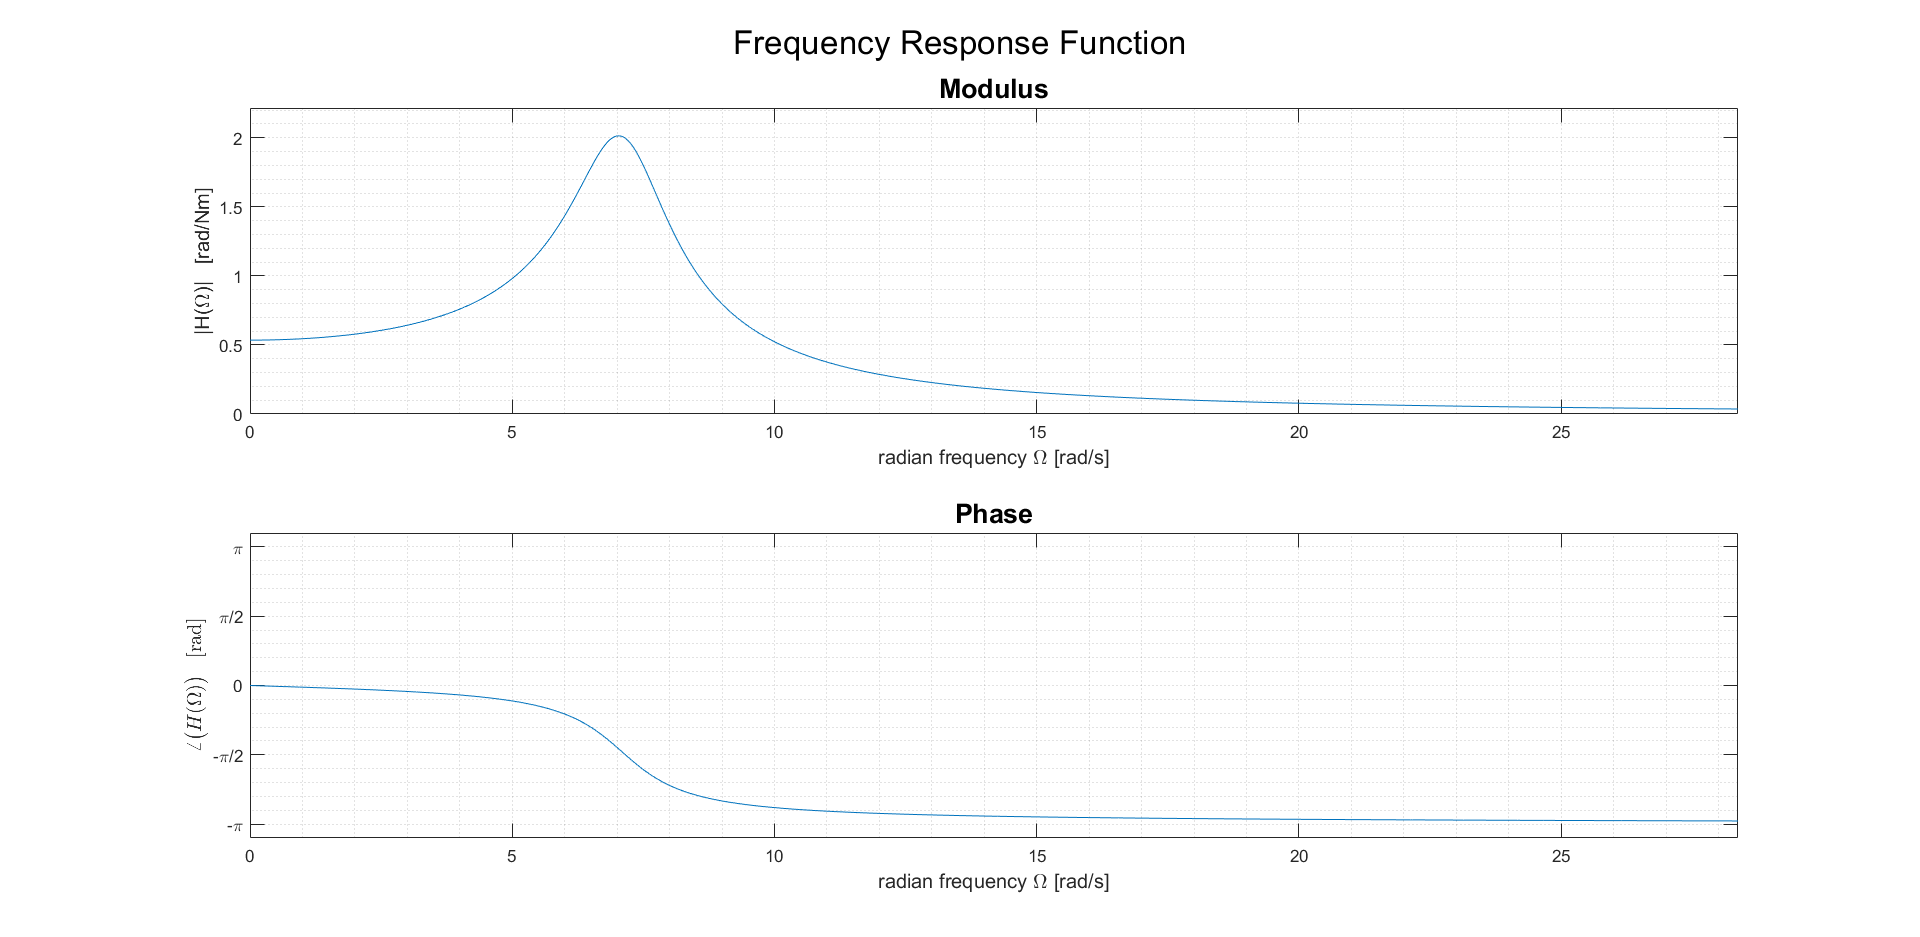
\includegraphics[scale=0.3]{frf.jpg}
\end{figure}

\subsubsection*{Case 2: halved adimensional damping ratio}

Considering half the damping ratio, we expect the system to be closer to the ideal undamped case, which means that the peak in the modulus diagram is going to be sharper than in the previous case (getting closer to the asymptotic behavior typical of the undamped system) and the phase jump suddener in the phase diagram (getting closer to the ideal perfectly vertical jump of the undamped case).

\begin{figure}
	\centering
	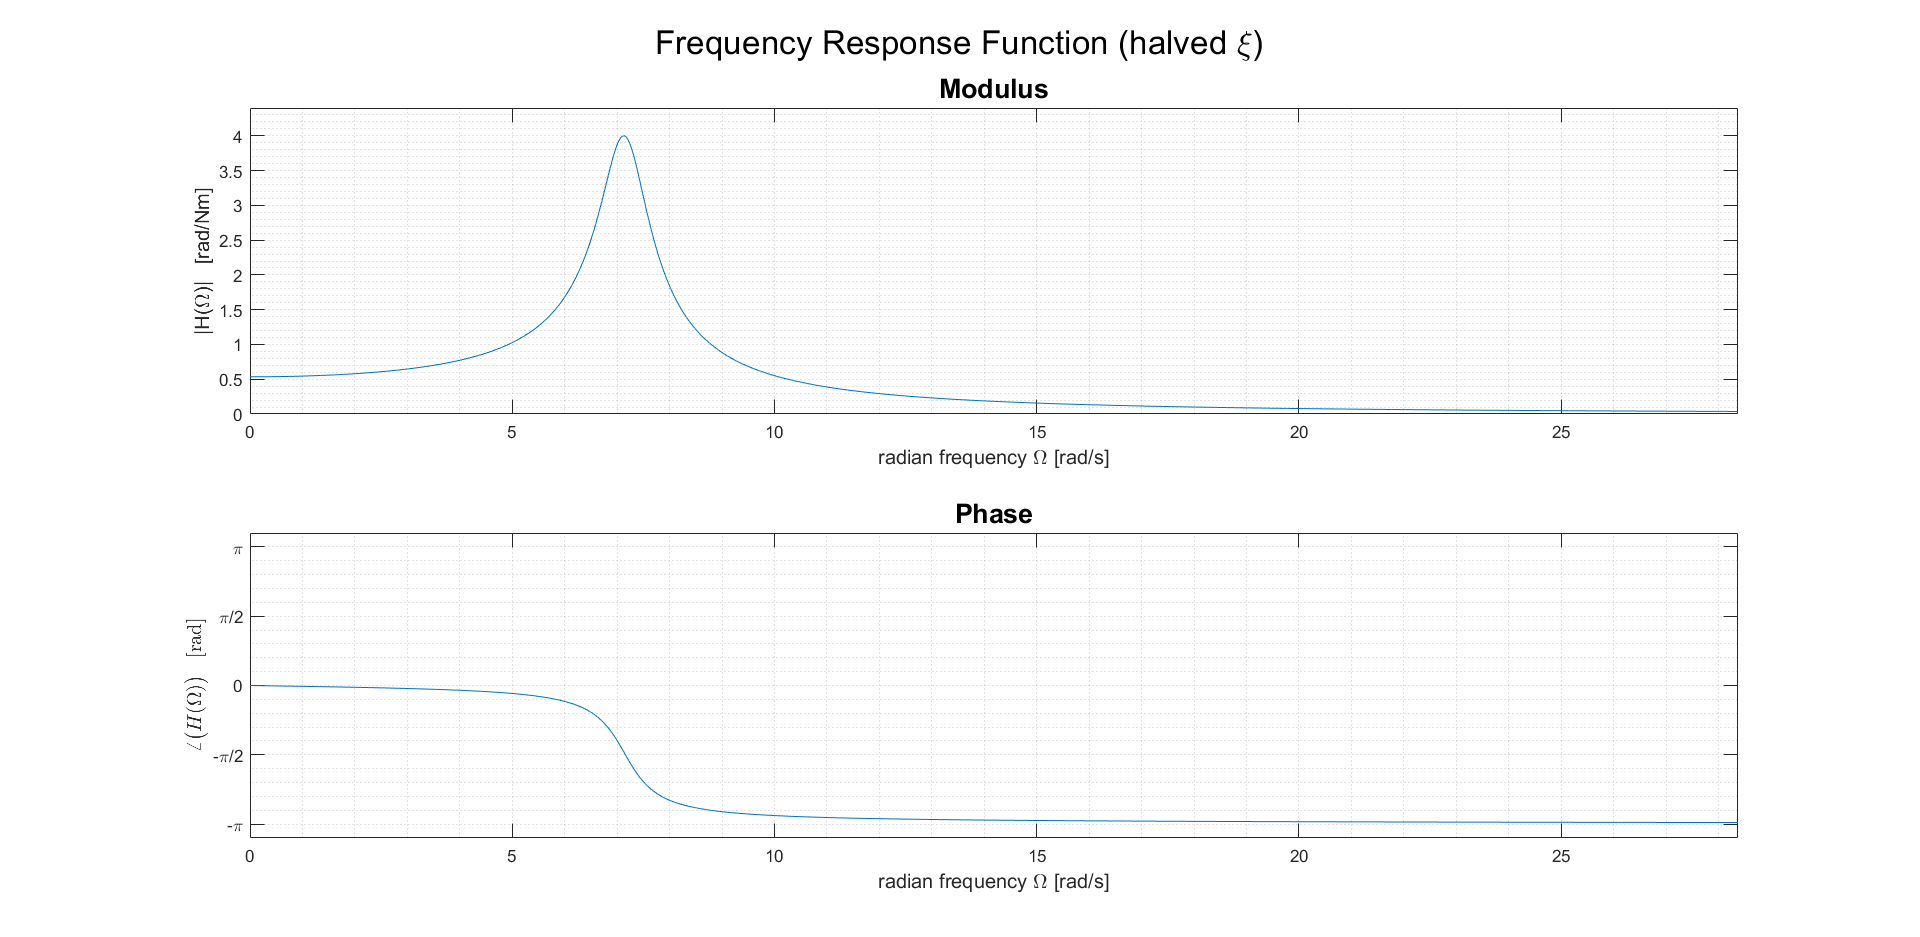
\includegraphics[scale=0.3]{frf_halved_damping_ratio.jpg}
\end{figure}

\subsubsection*{Case 3: raised adimensional damping ratio}

In this third case, the adimensional damping ratio is set to $ \xi = 1.2 $, so we find ourselves in the case of the overdamped system. We're not expecting a clear peak in the amplitude diagram as the damped natural frequency doesn't appear in the analytic formula of the time response, i.e. the system free motion does not oscillate, so the FRF shape is not depending on the natural frequency of the system. We might notice that the maximum steady-state oscillation amplitude is found for $ \omega = 0 $, i.e. for a constant external force.

\begin{figure}
	\centering
	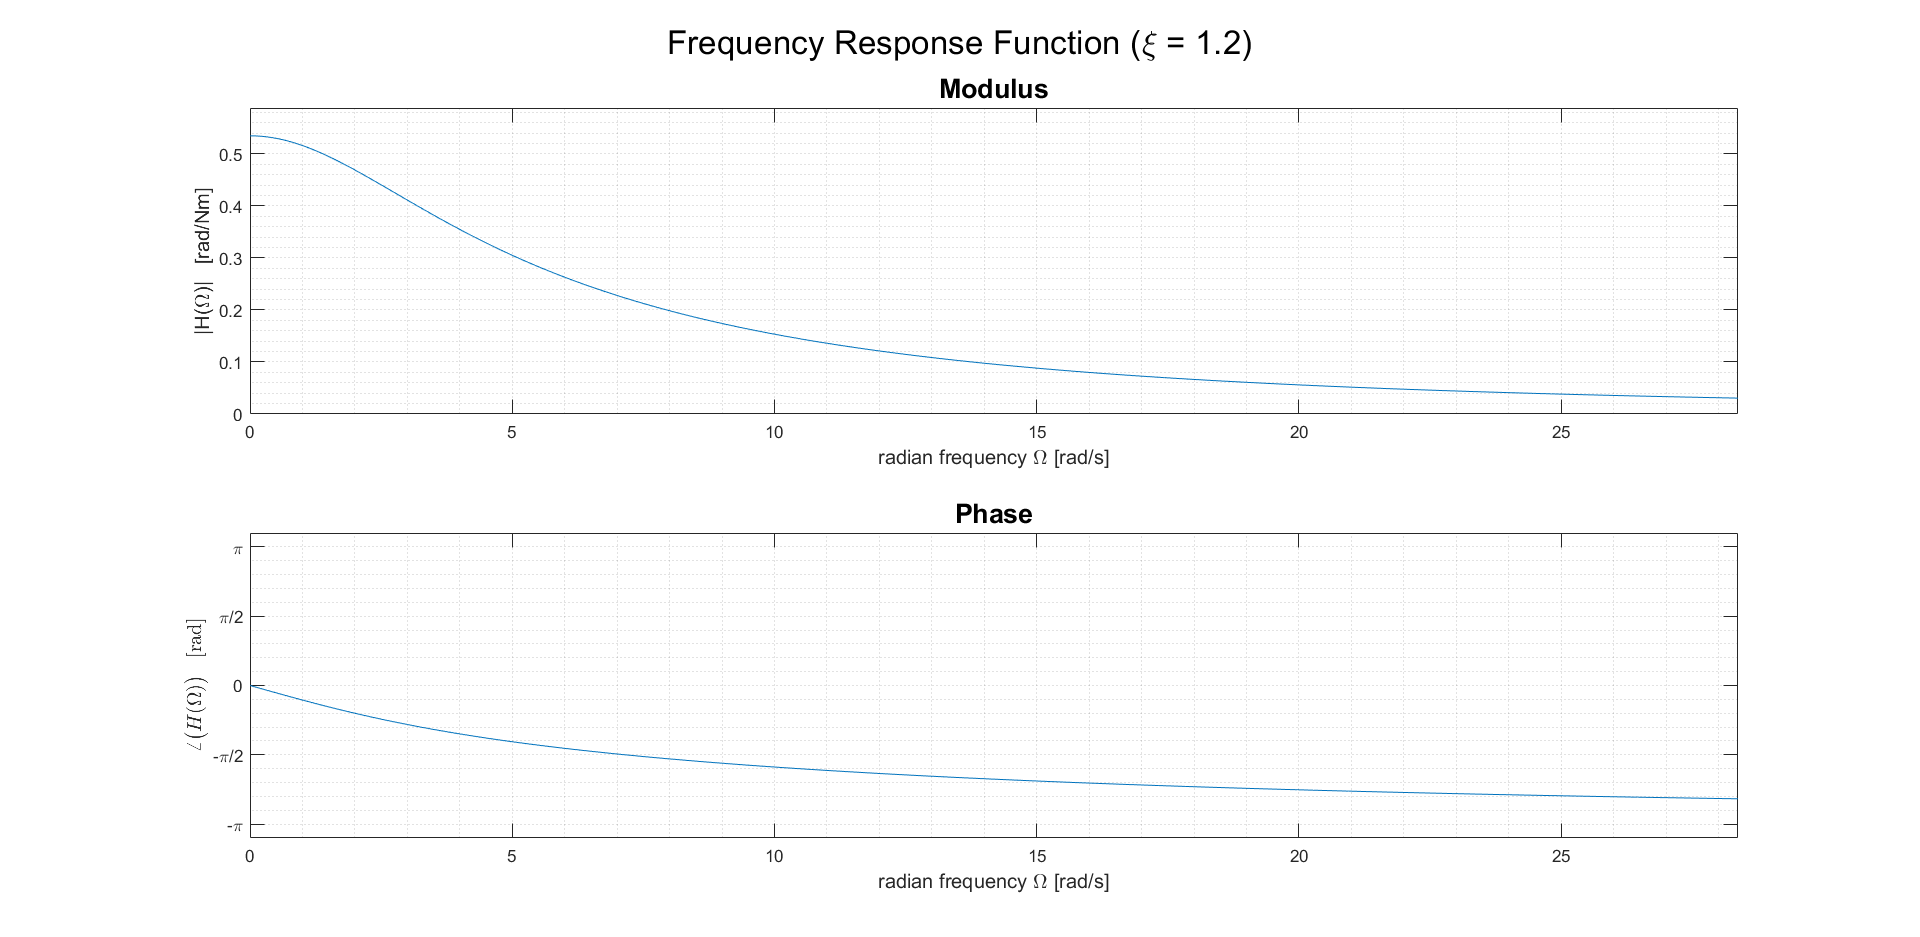
\includegraphics[scale=0.3]{frf_overdamped.jpg}
\end{figure}

\subsection{Temporal evolution of complete response of the system}

The system's complete response is composed by its free response and its forced response, summed together. The former is the one obtained in \ref{subs:generic_initial_conditions}. For the latter, the input force to the system is considered to be a harmonic force made up by a single sinusoidal wave:

\[ F = A \, cos(2 \pi f + \phi) \]

where $ A = 2.5 \, \text{N} $ and $ \phi = \frac{\pi}{3} $. We're considering two different cases for the frequency of this single harmonic component. In the first case

\[
	f = 0.15 \, \text{Hz} \Rightarrow %
	\omega = 2 \pi f \approx 0.94 \, \text{rad/s}
\]

while in the second

\[
	f = 4.5 \, \text{Hz} \Rightarrow %
	\omega = 2 \pi f \approx 28.27 \, \text{rad/s}
\]

 In each case, the steady-state motion has been computed by applying the well-known theoretical result stating the output of a linear time-invariant system is equal to the system input moduated in amplitude and phase by the FRF computed for the particular frequency $ \omega $ of the input:

\[
	x_{forced}(t) = |H(j \omega)| \, F_0 \, %
		cos\Bigl(\omega t + \phi + \angle\bigl(H(j \omega)\bigr)\Bigr)
\]

In our case, since the independent variable is an angle in radians, we need to divide this quantity by the radius $ R_2 $ that allows us to pass from the vertical dispacement $ y_2 $ of body $ M_2 $ to the disks rotation $ \theta $, so the final formula becomes

\[ \begin{split}
	\theta_{total}(t) & = \theta_{free} + \theta_{forced} = \\
										& = e^{-\alpha \, t} \, %
											(X_1 \, e^{j \omega_d \, t} + %
											X_2 \, e^{- j \omega_d \, t}) + %
											|H(j \omega)| \, \frac{F_0}{R2} \, %
											cos\Bigl(\omega t + \phi + %
											\angle\bigl(H(j \omega)\bigr)\Bigr)
\end{split} \]

We took the liberty of taking into account an additional case, where the external force frequency nearly matches the system's damped natural frequency, to check whether the amplitude of the resulting oscillation in steady-state is actually much larger than in the previous cases:

\[ \omega = 7 \, \text{rad/s} \]

The system's complete time responses for each of the three cases are shown in the following diagram.

\begin{figure}[h]
	\centering
	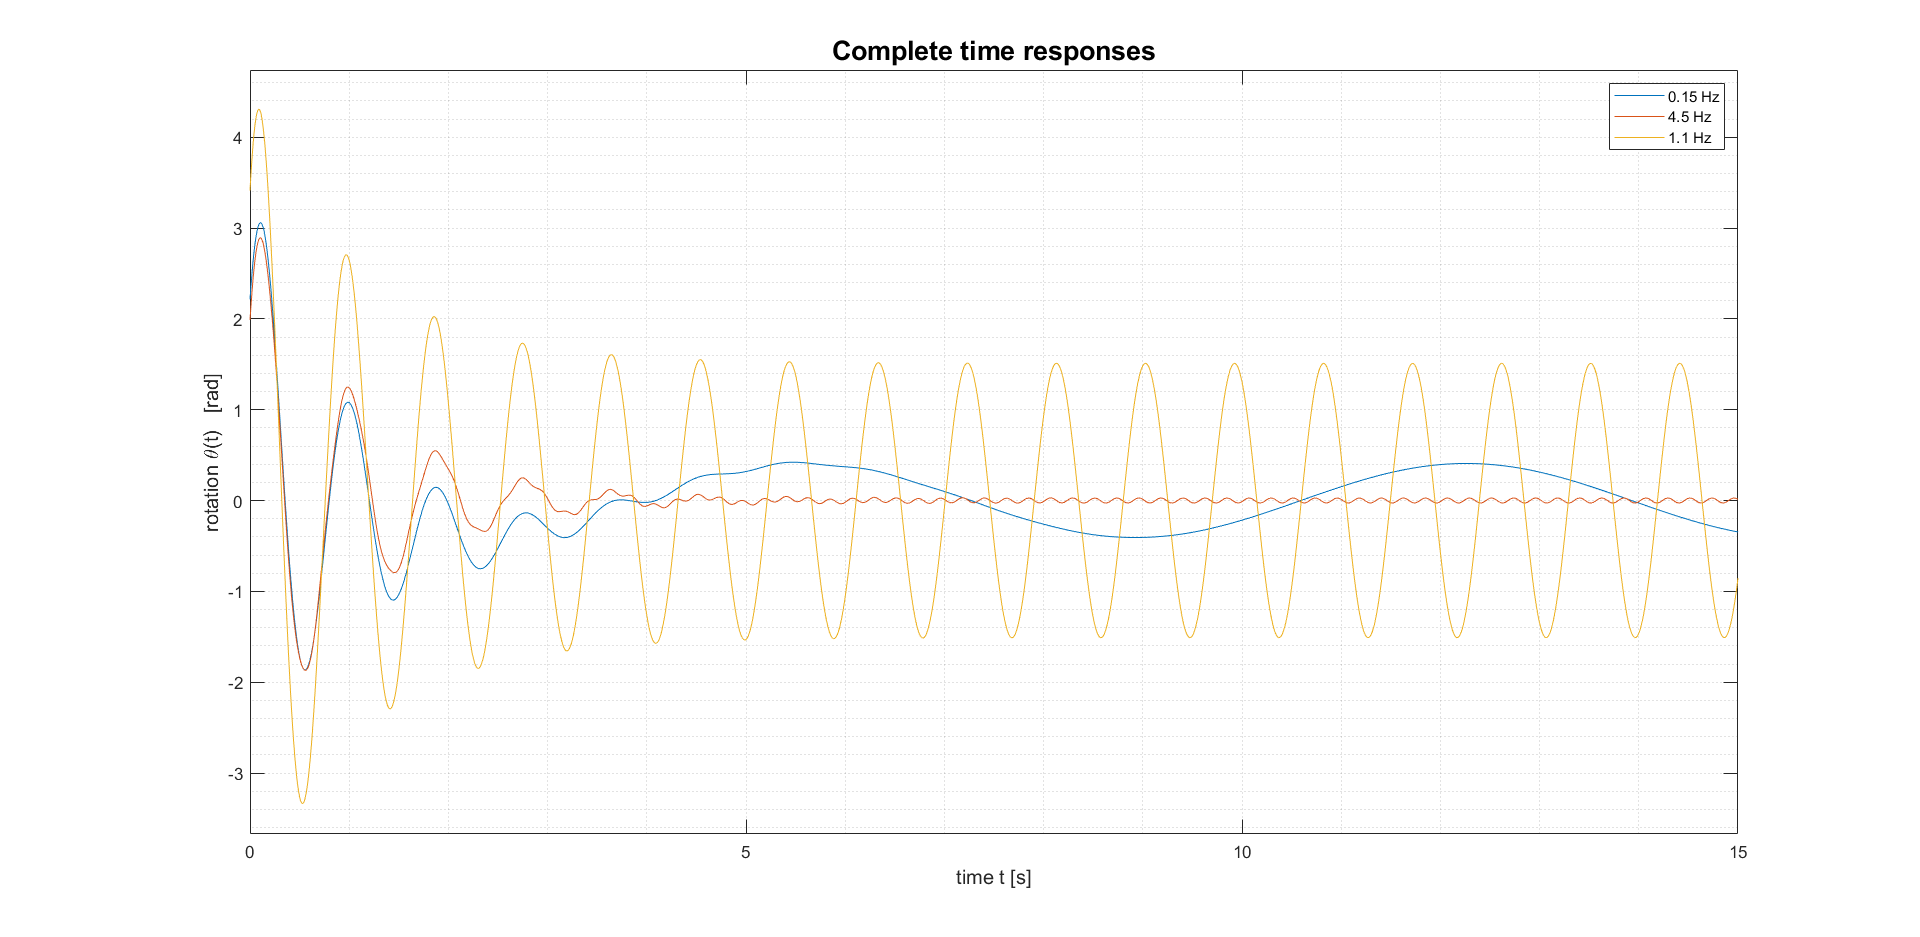
\includegraphics[scale=0.3]{complete_time_responses.jpg}
\end{figure}

\subsection{Forced response of the system (steady-state)}

Finally, let's consider this time a complex force composed by three harmonic components as system input:

\[ F(t) = \sum_{k=1}^3 B_k \, cos(2 \pi f_k t + \phi_k) \]

with $ B_1 = 1.2 \, \text{N} $, $ B_2 = 0.5 \, \text{N} $, $ B_3 = 5 \, \text{N} $, $ f_1 = 0.1 \, \text{Hz} $, $ f_2 = 0.6 \, \text{Hz} $, $ f_3 = 3.3 \, \text{Hz} $, $ \phi_1 = \frac{\pi}{4} $, $ \phi_2 = \frac{\pi}{5} $ and $ \phi_3 = \frac{\pi}{6} $. The external force and the forced vibration of the system are analyzed both in time and in frequency domain.

\begin{figure}
	\centering
	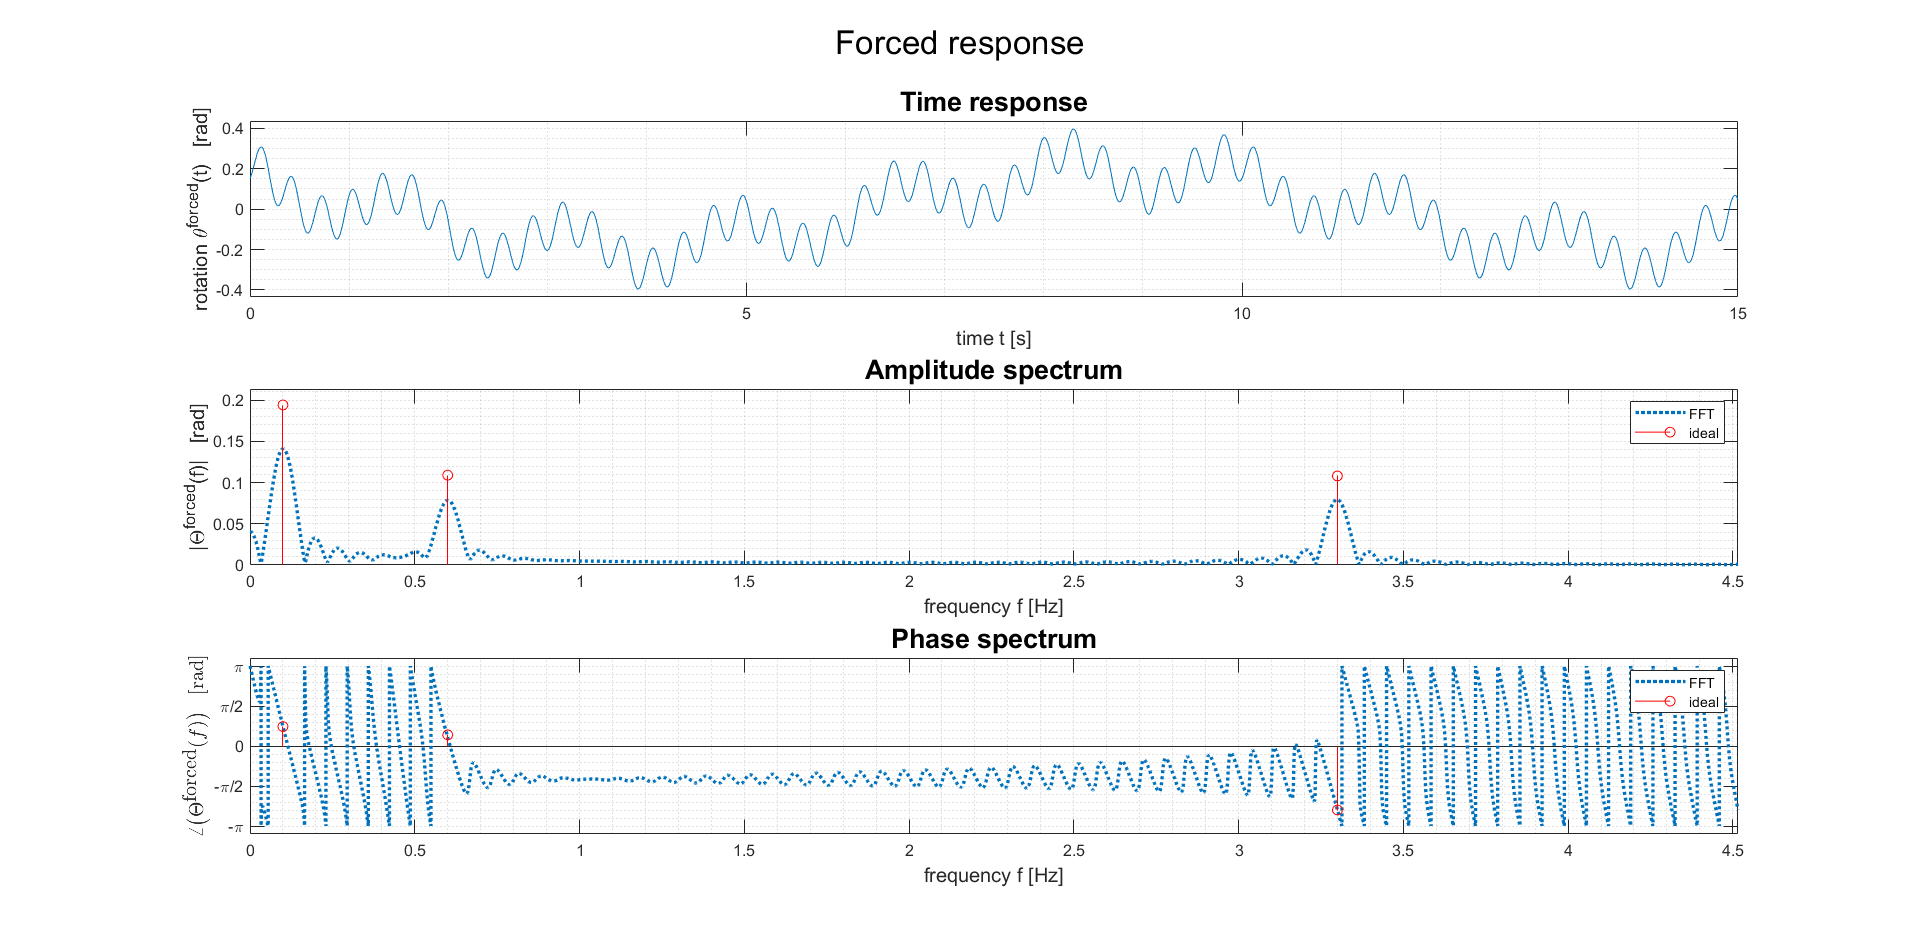
\includegraphics[scale=0.3]{forced_response.jpg}
\end{figure}

\begin{figure}
	\centering
	\includegraphics[scale=0.3]{complex_force.jpg}
\end{figure}


\end{document}
